\documentclass[aspectratio=169]{beamer}
\usetheme{hogent}
\usecolortheme{hgwhite} % witte achtergrond, zwarte tekst

%% common.tex -- Code die in elk .tex-bestand terug komt

%% Packages

\usepackage[dutch]{babel}
\usepackage{graphicx}
\usepackage{comment,enumerate,hyperref}
\usepackage{amsmath,amsfonts,amssymb}
\usepackage{eurosym}
\usepackage{booktabs}
\usepackage{multicol,multirow}
\usepackage{listings}

\usepackage[outputdir=out]{minted}
%\usepackage{minted}

\usepackage[backend=biber,style=apa]{biblatex}
\DeclareLanguageMapping{dutch}{dutch-apa}

\usepackage{csquotes}

%% Variabelen, elk academiejaar aan te passen
\newcommand{\academicyear}{2023--2024 (revisie: \today)}
\newcommand{\lecturers}{Thomas Aelbrecht \and Thomas Parmentier \and Bert Van Vreckem}
\newcommand{\coursename}{Research Methods (IT)}

%% Macro's en commando's

%% \alertbox: een kader voor tekst die moet opvallen
\newcommand{\alertbox}[2][hgblue]{%
  \setbeamercolor{alertbox}{bg=#1,fg=white}
  \begin{beamercolorbox}[sep=2pt,center]{alertbox}
    \textbf{#2}
  \end{beamercolorbox}
}


%---------- Info over de presentatie ------------------------------------------

\title{Module 6. Rapporteren over onderzoek in \LaTeX{}.}
\subtitle{Research Methods}
\author{\lecturers}   % Pas waarden aan in common.tex
\date{\academicyear}

\begin{document}

\begin{frame}
  \maketitle
\end{frame}

\begin{frame}
  \frametitle{Inhoud}

  \tableofcontents
\end{frame}

\section{Controle installatie}

\begin{frame}
  \frametitle{Heeft iedereen een werkende {\LaTeX}-installatie?}

  \begin{itemize}
    \item Compileert paper tot PDF?
    \item Is bibliografie zichtbaar? (F5-F8-F5)
    \item Correcte referenties in de tekst?
    \item Errors tijdens compilatie?
    \item Fouten in de PDF?
  \end{itemize}

\end{frame}

\begin{frame}
  \frametitle{Controleer:}

  \begin{itemize}
    \item Mik{\TeX} Console: controle op updates
      \begin{itemize}
        \item Als Administrator
        \item Als gewone gebruiker
      \end{itemize}
    \item Instellingen TeXstudio
      \begin{itemize}
        \item Compiler (\texttt{xelatex})
        \item Bibliografie (\texttt{biber}/\texttt{biblatex})
      \end{itemize}
  \end{itemize}

\end{frame}

\section{Korte tips}

\begin{frame}[fragile]
  \frametitle{Correct gebruik van aanhalingstekens}

  \textcolor{red}{\textbf{FOUT:}} \verb|"Een tekst"| $\Rightarrow$ \"Een tekst"

  \bigskip

  \textcolor{green}{\textbf{JUIST:}} \verb|``Een tekst''| $\Rightarrow$ ``Een tekst''

  \bigskip

  Gebruik twee ``backquotes'' (links) of twee enkele aanhalingstekens (rechts)
\end{frame}

\begin{frame}[fragile]
  \frametitle{URLs invoegen}

  \begin{itemize}
    \item Via package \texttt{hyperref} (al geladen in sjablonen!)
    \item Commando \verb+\url{}+, \verb+\href{}{}+
    \item Hyperref zorgt ook voor:
      \begin{itemize}
        \item Inhoudstafel in de PDF
        \item Aanklikbare verwijzingen binnen document
      \end{itemize}
  \end{itemize}

\end{frame}

\begin{frame}[fragile]
  \frametitle{URLs invoegen: voorbeeld}

  \verb+\url{https://xkcd.com/1301/}+ $\Rightarrow$ \url{https://xkcd.com/1301/}

  \bigskip

  \verb+\href{https://xkcd.com/1301/}{File Extensions}+ 
  
  $\Downarrow$
  
  \href{https://xkcd.com/1301/}{File Extensions}

\end{frame}

%% TODO:
% - Verwijzen naar hst, figuur, ... met \label en \ref

\section{Vlottende omgevingen}

\begin{frame}
  \frametitle{{\LaTeX} floating environments}

  \begin{itemize}
    \item = Inhoud die bij elkaar hoort, niet mag gesplitst worden
    \item Vb.\ afbeelding, tabel
    \item {\LaTeX} kiest waar ze geplaatst worden voor optimale bladspiegel
    \item Soms op andere bladzijde!
  \end{itemize}

\end{frame}

\begin{frame}
  \frametitle{Invoegen van afbeeldingen: fout}

  \centering
  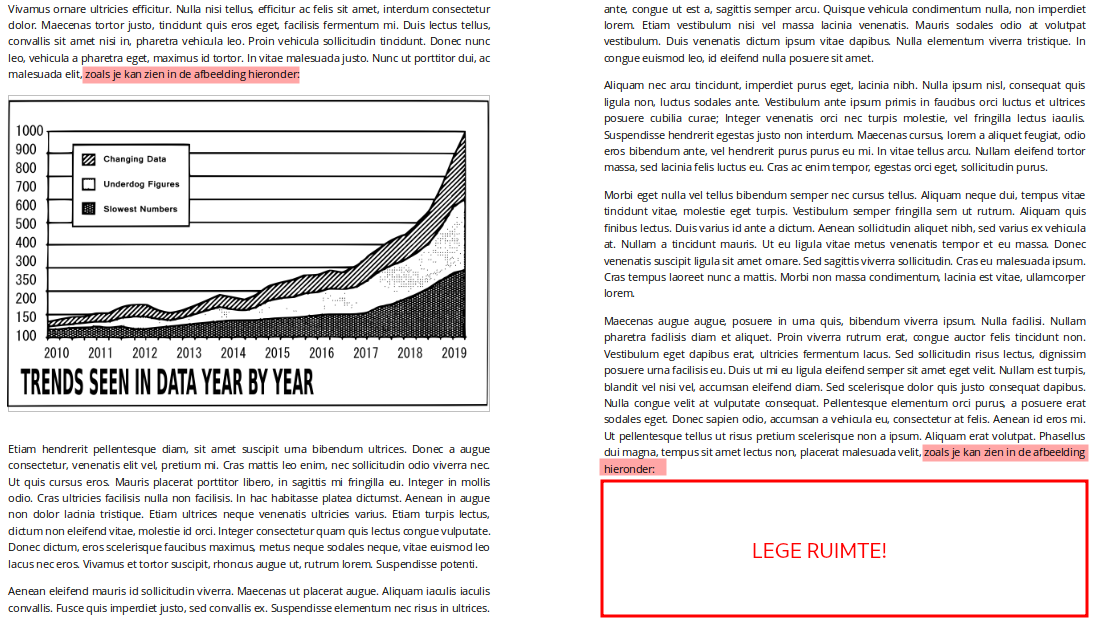
\includegraphics[height=.7\textheight]{6/afbeeldingen-tekstverwerker.png}

\end{frame}

\begin{frame}
  \frametitle{Afbeeldingen in {\LaTeX}}

  \begin{itemize}
    \item Gebruik Figure-omgeving
    \item Geef elke afbeelding een label
    \item Verwijs in de tekst naar de afbeelding
    \item Voorzie uitgebreide bijtekst (caption)
    \item Bronvermelding indien nodig!
  \end{itemize}

\end{frame}

\begin{frame}[fragile,plain]
  \frametitle{Afbeeldingen in {\LaTeX}}

  \begin{columns}[c]
    \column{.65\textwidth}
 
 \begin{semiverbatim}
 \alert<1>{\\begin\{figure\}}
 \alert<2>{\\includegraphics[width=\\textwidth]
   \{6/chart\}}
 \alert<3>{\\caption\{\alert<4>{\\label\{fig:chart\}}We zien jaar
   na jaar een stijgende trend in
   de data \alert<5>{\\autocite\{Doe2021\}}\}}
 \alert<1>{\\end\{figure\}}
 \end{semiverbatim}
 
    \column{.35\textwidth}
    \begin{figure}
      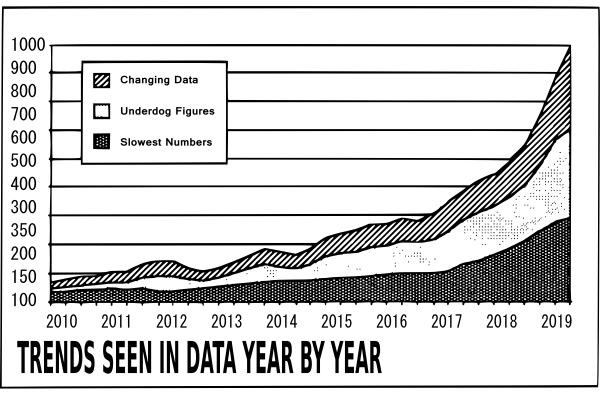
\includegraphics[width=\textwidth]{6/chart}
      \caption{\label{fig:chart}We zien jaar na jaar een stijgende trend in de data (Doe, 2021)}
    \end{figure}

  \end{columns}

\end{frame}

\begin{frame}[fragile]
  \frametitle{Verwijzingen in de tekst}

\begin{verbatim}
Volgens~\textcite{Doe2021} is er jaar na jaar een stijgende
trend waar te nemen (zie Figuur~\ref{fig:chart}).
\end{verbatim}

\[\Downarrow\]

\bigskip

Volgens Doe (2021) is er jaar na jaar een stijgende trend waar te nemen (zie Figuur 1.3).

\end{frame}

%% TODO
% - Tabellen: latextablegenerator, booktabs,
% - list of figures/tables
% - Wiskundige formules: basisprincipes, bruikbaarheid buiten LaTeX
% - Codefragmenten invoegen
% - optioneel: glossary?

\begin{frame}
  \frametitle{Tot slot: aanbevelingen}

  \begin{itemize}
    \item Bereid je tekst niet voor in Word om op het einde in {\LaTeX} om te zetten
    \item Begin met minimaal document dat compileert
    \item Werk stap voor stap, niet teveel tekst/code ineens toevoegen!
    \item \textbf{Lees aandachtig de foutboodschappen}
  \end{itemize}

% Stap over op een tekst-gebaseerde workflow
% Word in de vuilbak
% Markdown! Git! Pandoc! LaTeX!
% Idee: WSL installeren voor makkelijker beheer van alle nuttige Linux-tools

\end{frame}

\end{document}
